\documentclass[a4paper]{article}
\usepackage{amsfonts}
\usepackage{a4wide,times}
\usepackage[english]{babel}
\usepackage{graphicx}
\usepackage{listings}
\usepackage[parfill]{parskip}
\lstset{language=Java,
  numberstyle=\footnotesize,
  basicstyle=\footnotesize,
  numbers= left,
  stepnumber=1,
  tabsize=2,
  frame=shadowbox,
  breaklines=true
}


\begin{document}

\title{Net-computing\\
Architectural design document\\
Smart car on demand
}

\date{\today}

\author{Peri Rahamim (s2683423),\\
Jits Schilperoort (s2788659),\\
Twan Schoonen (s2756978)
}




\maketitle
\section*{Project description}
Smart car on demand is the name of our project idea to have self-driving cars drive through the city, and get ordered by customers who wish to go somewhere using this service. The order is done by a costumer logging in to a mobile application, and select their destination and number of passengers.

The request has the user's location saved, is sent to the car center, that selects the nearest car that can handle the request. Payment is done via money that is saved in the app account (top up is required beforehand). Requests are handled in queue order (first order-first served, maybe we add some priority).

The car arrives to the costumer(s) and takes them to their destination. Selecting a car and planning routes are handled by Artificial Intelligence systems that is able to compute the shortest route. The AI also allows the automated cars to drive without human intervention.

Since this is a big project, we will not implement all of the features, but only those relevant for this course. This list specifies the different elements of the system, with an explanation of why we decided to implement or not implement it:
\begin{itemize}
    \item \textbf{Mobile application:} Each costumer that is interested in getting a car to drive them uses a mobile app to make the order. A working app with an user friendly GUI is irrelevant for this course, so we decided to have a data structure that represents a user and has location, number of people who want to use the service, and destination instead.
    \item \textbf{AI:} The automated driving cars should know how to drive on roads without the help of humans. The AI of the car should follow the law and consider other cars (agents) or people crossing the road in its surrounding. This part is obviously too much to implement, and since it is also irrelevant to this course, we decided to assume the AI works.
    \item \textbf{Shortest distance algorithm:} We want the car to find the best route to reach its costumer, considering traffic and other parameters (such as construction that blocks the road). The algorithm helps deciding which car is most suitable to get to a costumer, in case there are more than one car in different parts of the city. To make this work we need live data, so for this project, we only send messages with datasets we made ourselves, and leave out the complicated calculations. The shortest distance is calculated using Pythagorean formula.
    \item \textbf{City layout:} To represent a city, we use a 100x100 plot along with number of rectangles representing building. Coordinates are represented as numbers 0-100 in the x and y axes. The city is divided to 4 areas, each has a unique color and its own car center. The map is drawn as an animation. Each frame draws the city map (same details as mentioned above), and retrieves locations of clients (marked as red points) and cars (marked as blue points) from object handler. 
    \item \textbf{Order handling:} The cars' and clients' locations are changed according to order handling in the following way: when a client sends an order, their location is shown on the map according to the coordinates of their location. If there are no available cars at the moment, the client waits. The available car with the shortest distance to the client goes to pick up the client, and changes its $isAvailable$ Boolean to False (initialized as True). When a client is picked up, they no longer appear on the map. The car, along with the client who is no longer represented on the map, goes to the clients destination. In case the destination belongs to a different center from where the car came from, the origin center that covers the area that the car came from, and the center that covers the area of the destination, update their cars lists, by removing the car from origin center's list, and adding it to new center's list. After arriving to the client's destination, the Boolean $isAvailable$ is changed to True, and the car returns to its (origin/new) center.
\end{itemize}

\section*{Project requirements}
The requirements that are implemented in this project are listed as follows:
\begin{itemize}
    \item \textbf{Socket:} used for center to car communication, also used for center to center communication. This is done when a destination is in an other center area then to location (longer drives).
    \item \textbf{Message queuing:} the requests made by the mobile application are queued by the centers, the when there are available cars the center dequeus the order and communicates with the car. 
    \item \textbf{Web services (REST):} the mobile app communicates with the database by using REST. This is used for getting client information.
\end{itemize}

\subsection*{Star vs P2P topology}
\textbf{Star topology:} The star topology is used by the centers to control the cars. Here the cars only drive and all computing is done by the center.\\
\textbf{P2P topology:} This method is used for center to center communication, so when a car leaves the district or city, the centers communicate to each other and swap cars.

\section*{Component diagram}
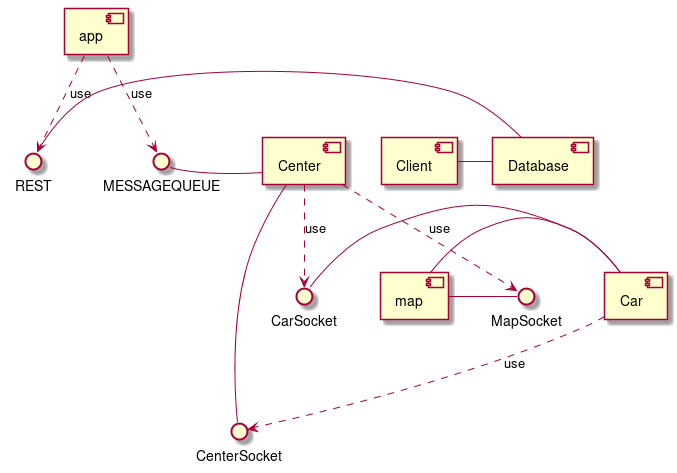
\includegraphics[width=1\textwidth]{../Diagrams/componentDiagram.png}

\section*{Class diagram}
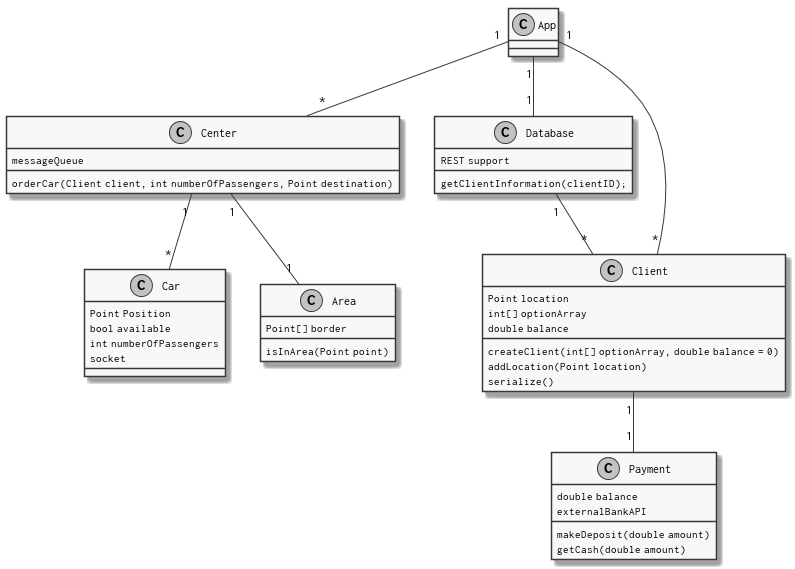
\includegraphics[width=1\textwidth]{../Diagrams/classDiagram.png}

\section*{Sequence diagrams}
\subsection*{RegisterClient}
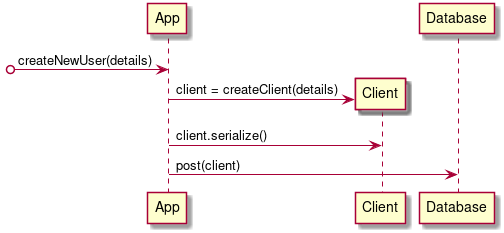
\includegraphics[width=1\textwidth]{../Diagrams/registerClient.png}\\
The client requests to sign up. App creates new object Client with the client's data that contains their personal preferences and money balance in the account. Client object is serialized and put in the database.

\subsection*{OrderCar}
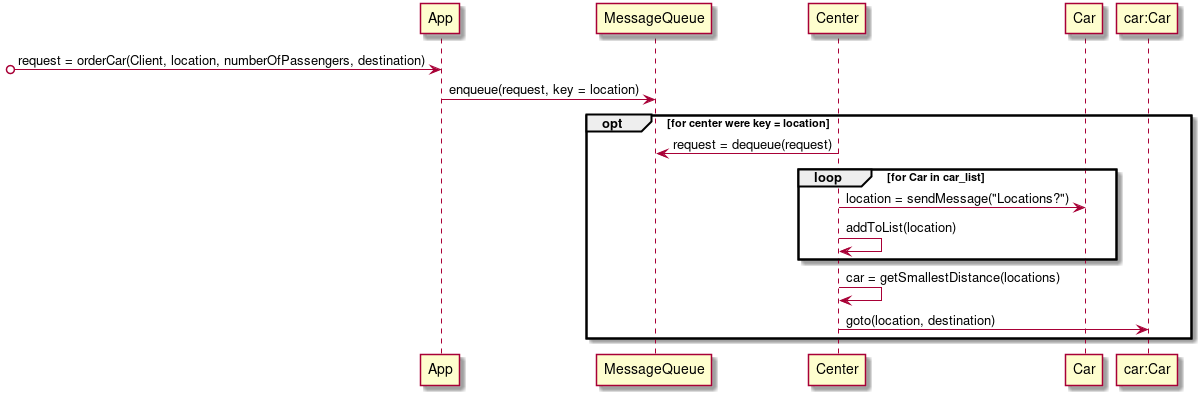
\includegraphics[width=1\textwidth]{../Diagrams/orderCar.png}\\
When a costumer orders a car, the app first checks in which area the costumer is, to know to which center it should send the order. The app then sends the order that has the object Client, the number of passengers, and the destination to the center. The center enqueues the order.
\subsection*{SendCar}
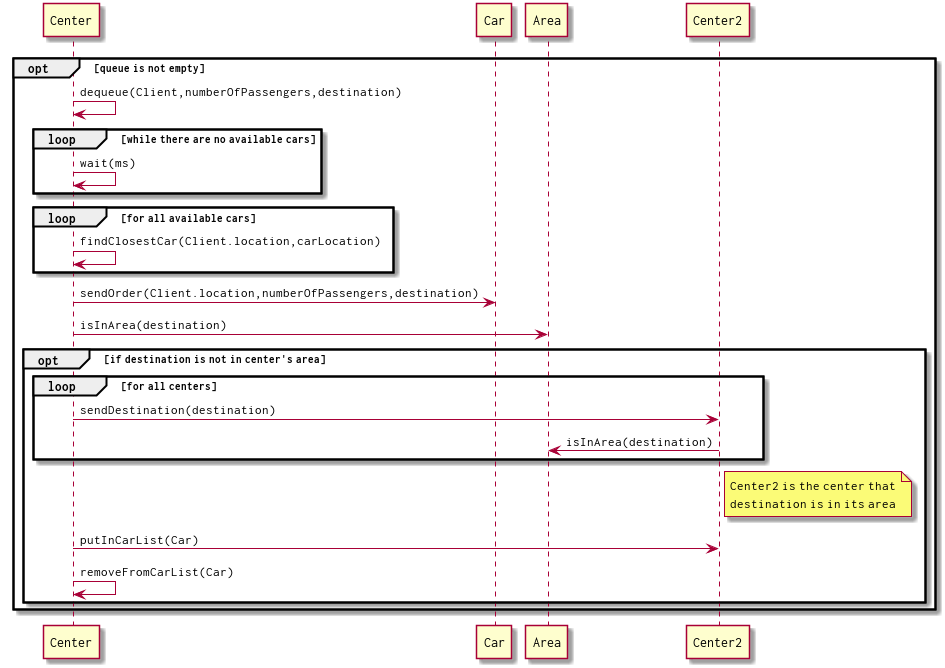
\includegraphics[width=1\textwidth]{../Diagrams/sendCar.png}\\
The entire use case starts only if queue is not empty. Center dequeues order. If there are no available cars, the center waits, and after this loop is terminated, it looks over the list of available cars, and finds the available car that is the closest to the client's location. The center sends the order to the car it found. The center checks if the destination is in its area, if not, the center sends the destination to all centers to check which one covers the area, and the car is removed from the list of the first center and entered to the list of the second center. 

\end{document}
